\chapter{Inflection points}

Traditionally, an \emph{inflection point}\define{inflection point} meant a point where the graph of a function changes from being convex down to being convex up, or vice versa.
Clearly at any inflection point, the derivative goes from decreasing to increasing, or vice versa, so the second derivative vanishes.
Notions of convexity depend very strongly on having some idea of positive and negative numbers, so they don't apply in the context of algebraic curves.
The closest we can come to this is to \emph{define} an \emph{inflection point} or \emph{flex}\define{flex} of an algebraic plane curve to be a point at which the tangent line meets the curve to order \(3\) or more.

To find such points, we define the \emph{Hessian} \(\Hessian{b}(x,y,z)\) of a homogeneous polynomial \(b(x,y,z)\) by
\[
\Hessian{b}(x,y,z) 
=
\det
\begin{pmatrix}
b_{xx} & b_{xy} & b_{xz} \\
b_{xy} & b_{yy} & b_{yz} \\
b_{xz} & b_{yz} & b_{zz} 
\end{pmatrix}
\]
where 
\[
b_{xy} \defeq \pderiv{b}{x,y}
\]
and so on.
If \(b(x,y,z)\) is homogeneous of degree \(n\), then \(b_{xy}\) is homogeneous of degree \(n-2\), so \(\Hessian{b}(x,y,z)\) is homogeneous of degree \(3(n-2)\).
\begin{example}
Take a conic \(B=(0=b(x,y,z))\), so \(b(x,y,z)\) has degree \(2\).
Then \(\Hessian{b}(x,y,z)\) is a constant, the determinant of the symmetric matrix of coefficients of \(b(x,y,z)\). 
Check that 
\[
2b(x,y,z)=
(x,y,z)
\begin{pmatrix}
b_{xx} & b_{xy} & b_{xz} \\
b_{xy} & b_{yy} & b_{yz} \\
b_{xz} & b_{yz} & b_{zz} 
\end{pmatrix}
\begin{pmatrix}
x\\
y\\
z
\end{pmatrix}.
\]
This determinant vanishes just when the matrix has a nonzero null vector, i.e. eigenvector of eigenvalue zero; arrange by linear change of \(x,y,z\) variables that this is \((0,0,1)\).
The Hessian matrix now has all second derivatives in \(z\) vanishing.
Suppose that the field is not of characteristic \(2\).
Then \(b(x,y,z)\) is independent of \(z\), so splits into linear factors over the algebraic closure by lemma~\vref{lemma:one.variable.splits}, i.e. into two linear factors, a pair of lines or a double line.
So over any field of characteristic \(2\), \(\Hessian{b}(x,y,z)\) is a nonzero constant just when \(b(x,y,z)\) is a smooth conic.
\end{example}
\begin{example}
Similarly, \(\Hessian{b}(x,y,z)\) vanishes everywhere for a double line or a pair of lines.
\end{example}
If the Hessian is not constant, the \emph{Hessian curve}\define{Hessian!curve} of the curve \(B=(0=b(x,y,z))\) is the curve \(H=(0=\Hessian{b}(x,y,z))\) of degree \(3(n-2)\).
\begin{example}
The Fermat curve \(F=(1=x^n+y^n)\) can be written homogenized as \((z^n=x^n+y^n)\), so as \((0=f)\) where 
\[
f(x,y,z)=x^n+y^n-z^n.
\]
The first derivatives are
\[
f_x=nx^{n-1},
f_y=ny^{n-1},
f_z=nz^{n-1}.
\]
Its Hessian is
\begin{align*}
\det f''(x,y,z)
&=
\det
\begin{pmatrix}
n(n-1)x^{n-2}&0&0\\
0&n(n-1)y^{n-2}&0\\
0&0&n(n-1)z^{n-2}
\end{pmatrix}
\\
&=n^3(n-1)^3(xyz)^{n-2},
\end{align*}
so vanishes exactly on the lines \((x=0)\), \((y=0)\), \((z=0)\).
The affine \(xy\)-plane picture for \(n=5\) is 
\includegraphicsinexample[width=4cm]{fermat5flexes}
and for \(n=6\):
\includegraphicsinexample[width=4cm]{fermat6flexes}
\end{example}
Sage can compute Hessians for us:
\begin{sageblock}
P.<x,y,z> = PolynomialRing(QQ)
b = x^3-y^2*z+z^3
Hb = matrix([[diff(b,x,x),diff(b,x,y),diff(b,x,z)],
             [diff(b,x,y),diff(b,y,y),diff(b,y,z)],
             [diff(b,x,z),diff(b,y,z),diff(b,z,z)]])
factor(Hb.det())
\end{sageblock}
yields \(\sage{latex(factor(Hb.det()))}\).
\begin{example}
Working over any field of characteristic \(3\), the polynomial \(b(x,y,z)\defeq x^3+y^3-z^3\) has derivatives \(0=b_x=b_y=b_z\), and so has Hessian \(\Hessian{b}(x,y,z)=0\).
\end{example}
\begin{problem}{inflection.points:Hessian.example}
Compute the Hessian of the curve \(y^2=x^3+x^2\) over any field.
For which characteristics is there are Hessian curve?
Very roughly, draw the curve and its Hessian curve, if the field is the real numbers.
\end{problem}
\begin{answer}{inflection.points:Hessian.example}
Let \(b(x,y)=y^2-x^3-x^2\), so homogenized: \(b(x,y,z)=y^2z-x^3-x^2z\).
\begin{align*}
b_x&=-3x^2-2xz,\\
b_y&=2yz,\\
b_z&=y^2-x^2,\\
\end{align*}
\begin{align*}
b''&=
\begin{pmatrix}
b_{xx}&b_{xy}&b_{xz}\\
b_{yx}&b_{yy}&b_{yz}\\
b_{zx}&b_{zy}&b_{zz}
\end{pmatrix},
\\
&=
\begin{pmatrix}
-6x-2z&0&-2x\\
0&2z&2y\\
-2x&2y&0
\end{pmatrix}
\end{align*}
Let 
\begin{align*}
h(x,y,z)
&=
\det b''(x,y,z),
\\
&=
(-6x-2z)
\det
\begin{pmatrix}
2z&2y\\
2y&0
\end{pmatrix}
-2x
\det
\begin{pmatrix}
0&2z\\
-2x&2y
\end{pmatrix},
\\
&=
(-6x-2z)(-4y^2)-2x(4z^2),
\\
&=
24xy^2+8y^2z-8xz^2,
\\
&=
8(y^2(3x+z)-xz^2).
\end{align*}
There is a Hessian curve just when this is not a constant, i.e. just when the field has characteristic not equal to \(2\).
Dehomogenize to \(z=1\): \(h(x,y)=8(y^2(3x+1)-x)\).
So \(H=(0=h(x,y)=(y^2(3x+1)=x)\).
Over the real numbers, we draw this as
\[
y=\pm\sqrt{\frac{x}{3x+1}},
\]
which has a vertical asymptote at \(x=-1/3\), and horizontal asymptotes at \(y=\pm 1/\sqrt{3}\).
It has no real points for \(-1/3<x<0\):
\[
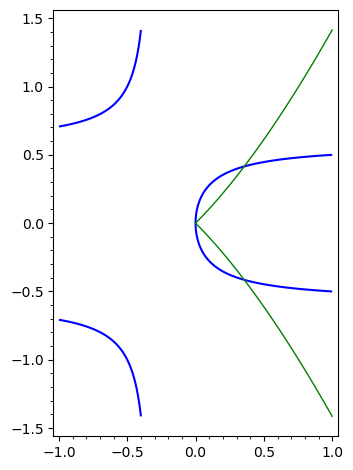
\includegraphics[width=5cm]{cuspidal-cubic-hessian}
\]
From the picture, there is clearly an inflection point at \(x=0\), and one positive real value of \(x\) where we find two inflection points.
Plugging in \(0=b=h\), we find 
\[
(x^3+x^2)(3x+1)=x,
\]
so \(x=0\) or 
\[
(x^2+x)(3x+1)=1.
\]
For \(x=0\), the left hand side is too small, but for \(x=1/2\) too large, it is too large, so by continuity, there is a root \(x\) with \(0<x<1/2\).
Expand out to find
\[
3x^3+4x^2+x=1.
\]
By Eisenstein's criterion, there are no rational roots.
The discriminant is negative, so there are two complex conjugate roots and there is one real root.
So in the affine \(xy\)-plane, there are two complex conjugate inflection points, one inflection point at the origin, and one real inflection point. 
\end{answer}
\begin{problem}{inflection.points}
Find the inflection points of the symmetric cubic curve, whose affine equation is
\[
x^3+y^3+1=3axy,
\]
over any field not of characteristic \(2\) or \(3\) and for \(a^3\ne 1\) (i.e. smooth).
\end{problem}
\begin{answer}{inflection.points}
Homogenize:
\[
b(x,y,z)=x^3+y^3+z^3-3axyz,
\]
and take Hessian
\[
b''(x,y,z)
=
\begin{pmatrix}
6x&-3az&-3ay\\
-3az&6y&-3ax\\
-3ay&-3ax&6z\\
\end{pmatrix}
\]
so
\[
\det b''(x,y,z)=-54(a^2(x^3+y^3+z^3)-(4-a^3)xyz).
\]
So the homogeneous equation of the Hessian curve of the Hesse curve is
\[
a^2(x^3+y^3+z^3)=(4-a^3)xyz.
\]
We get
\[
3a^3xyz=(4-a^3)xyz,
\]
and if \(x,y,z\ne 0\) this gives \(4a^3=4\) so \(a^3=1\), singular.
So \(x=0\) or \(y=0\) or \(z=0\), and then \(x^3+y^3+z^3=0\).
Trying each case, and recalling that rescaling a solution gives the same point of the projective plane, and writing the roots in \(\bar{k}\) of the equation \(\omega^3=-1\) as \(-1,\alpha,\beta\), we find that, up to permuting arbitrarily \(x,y,z\), our \(9\) distinct inflection points are
\[
\begin{bmatrix}
x\\
y\\
z
\end{bmatrix}
=
\begin{bmatrix}
0\\
1\\
-1
\end{bmatrix},
\begin{bmatrix}
0\\
1\\
\alpha
\end{bmatrix},
\begin{bmatrix}
0\\
1\\
\beta
\end{bmatrix},
\begin{bmatrix}
-1\\
0\\
1
\end{bmatrix},
\begin{bmatrix}
\alpha\\
0\\
1
\end{bmatrix},
\begin{bmatrix}
\beta\\
0\\
1
\end{bmatrix},
\begin{bmatrix}
1\\
-1\\
0
\end{bmatrix},
\begin{bmatrix}
1\\
\alpha\\
0
\end{bmatrix},
\begin{bmatrix}
1\\
\beta\\
0
\end{bmatrix}.
\]
\end{answer}
\begin{problem}{inflection.points:why.Hessian.1}
Take a projective transformation given by an invertible \(3\times 3\) matrix \(A\), over a field not of characteristic \(2\).
It is convenient to have a vector notation, say
\[
x=
\begin{pmatrix}
x_0\\
x_1\\
x_2
\end{pmatrix}
\]
Take any homogeneous polynomial \(b(x)\), say of degree \(d\).
Make new variables 
\[
X=
\begin{pmatrix}
X_0\\
X_1\\
X_2
\end{pmatrix}
\]
by
\[
\begin{pmatrix}
X_0\\
X_1\\
X_2
\end{pmatrix}
=
A
\begin{pmatrix}
x_0\\
x_1\\
x_2
\end{pmatrix}.
\]
Let \(c(X)=b(x)\).
So \(c(X)=0\) just where \(b(x)=0\), i.e. the plane algebraic curve \(C=(0=c(X))\) is just the image under the projective transformation of the curve \(B=(0=b(x))\); write this as \(C=A(B)\).
Show that the matrices of second derivatives at corresponding points are related by
\[
c''(X)=\left(A^{-1}\right)^tb''(x)A,
\]
(where \({}^t\) means transpose).
Show that the Hessian curves are also related by \(H_C=A(H_B)\).
\end{problem}
\begin{answer}{inflection.points:why.Hessian.1}
In a Taylor series
\[
b(x+y)=b(x)+\text{linear terms in \(y\)}+\text{quadratic terms in \(y\)}+\dots,
\]
with finitely many terms, because it is a polynomial.
The quadratic terms are of course \(y^tb''(x)y\) so ignoring terms of all degrees but quadratic:
\[
b(x+y)=\dots+y^t b''(x_0,y_0,z_0)y+\dots.
\]
In the same way,
\[
c(X+Y)=\dots+
Y^t
c''(X)
Y+\dots.
\]
But \(b(x)=c(X)\) and \(X=Ax\) and so \(Y=Ay\) giving
\[
y^tb''(x)y=(Ay)^tc''(x)Ay=y^tA^tc''(x)Ay.
\]
This holds for all \(y\) and the matrices are symmetric; expand out in entries of \(y\) to find
\[
b''(x)=A^tc''(x)A.
\]
Take determinants to find
\[
\det b''(x)=(\det A)^2\det c''(X),
\]
and so \(0=\det c''(X)\) just when \(0=\det b''(x)\).
\end{answer}
\begin{lemma}[Euler]\label{lemma:Euler}\SubIndex{lemma!Euler}\SubIndex{Euler!lemma}
Every homogeneous polynomial \(b(x,y,z)\), say of degree \(n\), over any commutative ring with identity, satisfies
\[
nb(x,y,z)=x \pderiv{b}{x} + y \pderiv{b}{y} + z \pderiv{b}{z}.
\]
\end{lemma}
\begin{proof}
Since \(b(x,y,z)\) is a sum of homogeneous terms, it is enough to check one such term, which is easy for the reader to check.
\end{proof}
\begin{lemma}\label{lemma:H.zero.at.flex}
The Hessian \(\Hessian{b}(x,y,z)\) vanishes at a smooth point of a plane algebraic curve \(B=(0=b(x,y,z))\) just when that point is a flex of \(B\).
\end{lemma}
\begin{proof}
Euler's lemma:
\[
nb(x,y,z)=x \pderiv{b}{x} + y \pderiv{b}{y} + z \pderiv{b}{z}
\]
applies to the homogeneous polynomials \(b_x \defeq \pderiv{b}{x}\) and so on to yield
\begin{align*}
(n-1)b_x &= x b_{xx} + y b_{xy} + z b_{xz}, \\
(n-1)b_y &= x b_{xy} + y b_{yy} + z b_{yz}, \\
(n-1)b_z &= x b_{xz} + y b_{yz} + z b_{zz}.
\end{align*}
Multiply row 1 of the Hessian determinant by \(x\), row 2 by \(y\), and add to the third row multiplied by \(z\) to get
\[
z \Hessian{b}(x,y,z)=(n-1) 
\det
\begin{pmatrix}
b_{xx} & b_{xy} & b_{xz} \\
b_{xy} & b_{yy} & b_{yz} \\
b_x & b_y & b_z 
\end{pmatrix}.
\]
Apply the same trick across the columns instead of the rows:
\begin{equation}\label{equation:z2H}
z^2 \Hessian{b}(x,y,z)=(n-1)^2
\det
\begin{pmatrix}
b_{xx} & b_{xy} & b_x \\
b_{xy} & b_{yy} & b_y \\
b_x & b_y & \frac{n b}{n-1}
\end{pmatrix}.
\end{equation}
At singular points of the curve \(B=(0=b(x,y,z))\), the final row vanishes, so the determinant vanishes.
At any point where the curve \(B=(0=b(x,y,z))\) is not singular, which we can arrange that point to be \((x,y,z)=(0,0,1)\).
Arrange that the tangent line of \(B\) at that point is the \(x\)-axis, so \(b_y=1\) while \(b_x=0\).
Euler's lemma gives \(b_z=0\).
Plug into equation~\vref{equation:z2H} to get \(\Hessian{b}(0,0,1)=(n-1)^2 b_{xx}(0,0,1)\).
The multiplicity of \(b\) restricted to \(x=0\) is then given by expanding out \(b(0,y)=b(0,0)+b_y(0,0)y+b_{yy}(0,0)y^2/2+\dots\), clearly at least 3.

By implicit differentiation, at any smooth point, the slope of the tangent line is
\[
0 = b_x+b_y y'
\]
and so differentiating again gives
\[
0 = b_{xx} + 2 b_{xy} y' + b_{yy} (y')^2 + b_y y'',
\]
as the derivative of \(y'\).
So
\[
y'=-\frac{b_x}{b_y}, 
\]
while
\[
y''=-\frac{b_{xx} + 2 b_{xy} y' + b_{yy} (y')^2}{b_y}.
\]
Expanding out,
\begin{align*}
y''
&=\frac{-b_{xx} b_y^2 + 2b_{xy} b_x b_y - b_{yy}b_x^2}{b_y^3},
\\
&=\frac{1}{b_y^3} 
\begin{pmatrix}
b_{xx} & b_{xy} & b_x \\
b_{xy} & b_{yy} & b_y \\
b_x & b_y & 0
\end{pmatrix}
\end{align*}
So at any point where \(b=0\), this is
\[
y''
=
\frac{\Hessian{b}(x,y,1)}{(n-1)^2 b_y^3}.
\]
If we take a point \((x_0,y_0)\) at which \(b_y \ne 0\), let \(y'_0\) be \(y'\) at that point, and compute out that on the tangent line,
\begin{align*}
b(x,y)&=b(x_0+\Delta x,y_0+y_0' \Delta x),
\\
&= b(x_0,y_0)+b_x(x_0,y_0)\Delta x + \dots,
\\
&=-b_y(x_0,y_0) y_0'\Delta x -b_y(x_0,y_0) y''_0 \frac{\Delta x}{2} + \dots
\end{align*}
So the Hessian vanishes just where the tangent line meets the curve to order \(3\) or more, and this occurs just where \(y''=0\).
\end{proof}

\begin{lemma}\label{lemma:vanishing.Hessian}
Take a plane algebraic curve \(B=(0=b(x,y,z))\).
Suppose that the characteristic of the field is zero or coprime to the exponents appearing in all terms of \(b(x,y,z)\).
Then \(b(x,y,z)\) has vanishing Hessian just when \(B\) is a union of lines.
In other words, \(B\) has Hessian curve \(H\) defined just when \(B\) is not a union of lines.
\end{lemma}
\begin{proof}
Continuing the previous proof, if we suppose that the Hessian vanishes everywhere, we see that \(y''\) is everywhere zero, i.e. we see that at every point where \(b=0\),
\[
0 = y''=(y')_x + (y')_y y'.
\]
Plug in \(y'=-b_x/b_y\) to get
\[
\pr{\frac{b_x}{b_y}}_x = \pr{\frac{b_x}{b_y}}\pr{\frac{b_x}{b_y}}_y.
\]
This last equation turns a derivative in \(x\) into a product, with the first factor having no derivative in \(x\).
Note that it only holds at points of the curve, so holds modulo \(b\).
Hence, when we differentiate both sides, the result hold modulo \(b,b_x\), and so on.
By induction, at a point where \(0=b=b_x\) and where \(0 \ne b_y\), if we differentiate both sides repeatedly, we find a higher order \(x\) derivative of \(b\) vanishing each time.
So at any point where \(0=b=b_x\) we also have \(0=b=b_x=b_{xx}=\dots\).
Because the exponents arising in the terms of \(b(x,y,z)\) are coprime to the characteristic of the field, the vanishing of derivatives \(b_x,b_{xx},\dots\) implies that the coefficients of \(x,x^2,\dots\) in \(b(x,y,1)\) are zero.
Every term in \(b\) contains a factor of \(y\), so \(b=0\) along the line \(y=0\).
\end{proof}
\begin{lemma}\label{lemma:Hessian.multiplicity}
Take a plane algebraic curve \(B=(0=b(x,y,z))\) with Hessian curve \(H\).
Let \(n\) be the degree of \(B\).
Then \(H\) passes through all singular points of \(B\), intersecting \(B\) at \(3n(n-2)\) points at most, counting with multiplicity.
The curves \(H\) and \(B\) share no component.
Moreover, \(H\) meets \(B\) at a smooth point of \(B\) with multiplicity \(r\) just when the tangent line at that point meets \(B\) with multiplicity \(r+2\).
\end{lemma}
\begin{proof}
We can assume that the point in question is the origin in the affine plane, and that the tangent line is \(y=0\).
Factoring out all copies of \(x\) from the terms with no \(y\) in them, the equation of \(B\) is now
\[
0=b(x,y)=y \, f(x,y) + x^{r+2} g(x),
\]
with \(f(0,0)\ne 0\) and \(g(0) \ne 0\).
We can rescale \(x,y\) to arrange \(f(0,0)=1\) and \(g(0)=1\).

The associated homogeneous polynomial is 
\[
b(x,y,z) = y \, f(x,y,z) +  x^{r+2} g(x,z).
\]
Note that the affine equations \(f(0,0)=1\) and \(g(0)=1\) become homogeneous equations \(f(0,0,z)=z^{n-1}\) and \(g(0,z)=z^{n-r-2}\).
The Hessian \(\Hessian{b}(x,y,z)\) is extremely complicated in terms of \(f, g\).
The first derivatives are
\begin{align*}
b_x 
&= 
yf_x + (r+2)x^{r+1}g + x^{r+2} g_x,
\\
b_y
&= 
f+yf_y + x^{r+2} g_y,
\\
b_z
&= 
yf_z + x^{r+2} g_z,
\end{align*}
and the second derivatives are
\begin{align*}
b_{xx} 
&=
yf_{xx}
+
(r+2)(r+1)x^r g
+
2(r+2)x^{r+1}g_x
+
x^{r+2} g_{xx},
\\
b_{xy}
&=
f_x
+
yf_{xy}
+
(r+2)x^{r+1}g_y
+
x^{r+2}
g_{xy},
\\
b_{xz}
&=
yf_{xz} + (r+2)x^{r+1}g_z + x^{r+2} g_{xz},
\\
b_{yy}
&=
2f_y + yf_{yy} + x^{r+2}g_{yy},
\\
b_{yz}
&=
f_z + yf_{yz} + x^{r+2} g_{yz},
\\
b_{zz} 
&=
yf_{zz} + x^{r+2} g_{zz}.
\end{align*}

Modulo \(y,x^r\), i.e. dropping terms with \(y\) or \(x^r\) in them, we find
\[
\Hessian{b}(x,y,z)
=
\det
\begin{pmatrix}
0 & f_x & 0 \\
f_x & 2f_y & f_z \\
0 & f_z & 0
\end{pmatrix}=0.
\]
So every term in \(\Hessian{b}(x,y,z)\) contains either \(y\) or \(x^r\):
\[
\Hessian{b}(x,y,z)=yF(x,y,z)+x^rG(x,y,z)
\]
for some polynomials \(F,G\).
We can absorb any \(y\) terms in \(G\) into \(F\), so 
\[
\Hessian{b}(x,y,z)=yF(x,y,z)+x^rG(x,z)
\]
for some polynomials \(F,G\).
Compute \(\Hessian{b}(x,y,z)\) modulo \(y\), and divide out \(x^r\) from the first row, and then set \(x=0\), to find
\[
G(0,1)=
\frac{\Hessian{b}}{x^r}(0,0,1)=
-{\left(r + 2\right)} 
{\left(r + 1\right)} 
g\left(0, 1\right) 
f_z\left(0, 0, 1\right)^2.
\]
We can actually get sage to compute this for us:
\begin{sageblock}
y=var('y')
z=var('z')
r=var('r')
f = function('f')(x,y,z)
g = function('g')(x,z)
b(x,y,z) = y * f + x^(r+2)*g
m=matrix([
        [diff(b(x,y,z),x,x),diff(b(x,y,z),x,y),diff(b(x,y,z),x,z)],
        [diff(b(x,y,z),x,y),diff(b(x,y,z),y,y),diff(b(x,y,z),y,z)],
        [diff(b(x,y,z),x,z),diff(b(x,y,z),y,z),diff(b(x,y,z),z,z)]])
h=m.det()
factor(simplify(expand((h.subs(y=0)/x^r).subs(x=0))))
\end{sageblock}
prints out \(\sage{latex(factor(simplify(expand((h.subs(y=0)/x^r).subs(x=0)))))}\).
(The sage notation for derivatives is peculiar, and we leave the reader to work out why \(D_2\) means derivative in the third variable.)
Since we know that \(f(0,0,z)=z^{n-1}\) and \(g(0,0,1)=1\), we can compute out
\[
G(0,1)=
\frac{\Hessian{b}}{x^r}(0,0,1)=
-{\left(r + 2\right)} 
{\left(r + 1\right)} 
(n-1)^2.
\]
Returning to affine coordinates, at the origin \((x,y)=(0,0)\) in the \((x,y)\) affine plane,
\[
G(0)=-{\left(r + 2\right)}{\left(r + 1\right)}(n-1)^2 \ne 0.
\]

We are looking for \(H \cap B\) near the origin \((0,0,1)\), i.e. we are looking for common zeroes, with multiplicity, of 
\begin{align*}
0 &= yf(x,y,z)+x^{r+2}g(x,z), \\
0 &= yF(x,y,z)+x^rG(x,z).
\end{align*}
Dehomogenize by setting \(z=1\):
\begin{align*}
0 &= yf(x,y)+x^{r+2}g(x), \\
0 &= yF(x,y)+x^rG(x).
\end{align*}
If \(r=0\), then the second equation doesn't vanish near \((x,y)=(0,0)\), so the origin is not an intersection point, contradicting our assumptions.
So \(r\ge 1\).

Suppose that \(B\) and \(H\) share a common component, and suppose that the origin belongs to that component.
If \(y=0\) on some intersection point, then plug in to get that either \(x=0\) or \(g(x)=0\).
But \(g(0)=1\), so \(g(x)\) is zero at only finitely many points, none near the origin.
The same holds over any algebraic extension of our field.
So \((y=0)\) is not a component of \(B \cap H\), i.e. if \(B \cap H\) contains a curve, it is not inside the line \((y=0)\).
Solve for \(x^r\) as
\[
x^r=\frac{y}{(r+1)(r+2)(1+\dots)},
\]
and plug in to get
\[
\frac{x^2 y}{(r+1)(r+2)(1+\dots)} = -y\frac{1+\dots}{1+\dots}.
\]
Cancel the \(y\), since \((y=0)\) is not in \(B \cap H\):
\[
x^2 = -(r+1)(r+2)\frac{1+\dots}{1+\dots},
\]
and clear denominators:
\[
x^2(1+\dots)=-(r+1)(r+2)(1+\dots).
\]
on any common component of \(B\) and \(H\).
But this is not satisfied at the origin, so the common component does not meet the origin.
Recall that we picked any point of \(H \cap B\) and made it the origin.
Hence \(B\) and \(H\) share no common component.

We will compute the multiplicity of intersection \(\multiplicity{p}{B}{H}\) at any smooth point \(p\) of \(B\).
We can assume that we have chosen very generic affine coordinates, so that the line through any two intersection points of \(B\) and \(H\) does not touch \((0,1)\) (even after an algebraic extension of the field).
We can still arrange that \(p\) is the origin \((0,0)\) and that the tangent line to \(B\) at \((0,0)\) is \(y=0\).
Take the resultant \(R(x)\) of \(yf(x,y)+x^{r+2}g(x)\) and \(yF(x,y)+x^rG(x)\).
By theorem~\vref{theorem:intersection.number.definition},  \(\multiplicity{p}{B}{H}\) is the order of vanishing of \(R(x)\) at the origin: if we write
\begin{align*}
f(x,y)&=\sum y^j f_j(x), \\
F(x,y)&=\sum y^j F_j(x),
\end{align*}
then
\[
R(x)
=
\det
\begin{pmatrix}
x^{r+2}g(x)   &               &        &             & x^r G(x)   \\
f_1(x)        & x^{r+2} g(x)  &        &             & F_1(x)       & x^rG(x)  \\
\vdots        & f_1(x)        & \ddots &             & \vdots       & F_1(x)      & \ddots  & \\
f_k(x)        & \ddots        & \ddots & x^{r+2}g(x) & F_{\ell}(x)  & \ddots      & \ddots  & x^rG(x) \\
              & f_k(x)        & \ddots & f_1(x)      &              & F_{\ell}(x) & \ddots  & F_1(x) \\
              &               & \ddots & \vdots      &              &             & \ddots  & \vdots \\
              &               &        & f_k(x)      &              &             &         & F_{\ell}(x)
\end{pmatrix}.
\]
Expand across the top row to see that \(R(x)\) is a multiple of \(x^r\).
We want to prove that \(R(x)\) has order exactly \(x^r\), no something higher.
The \(x^r\) term in \(R(x)\) doesn't notice terms of order \(x^{r+1}\) or higher, so we can assume that \(g(x)\) and \(G(x)\) are constants, both equal to \(1\).
Terms of higher order than \(x^r\) make no contribution to the order \(r\) term in \(R(x)\), so we only need to find the resultant of \(yf(x,y),yF(x,y)+x^r\).
If we write dots to indicate terms of higher order than \(x^r\),
\begin{align*}
R(x)
&=
\resultant{yf(x,y)}{yF(x,y)+x^r} + \dots,
\\
&=\resultant{y}{yF(x,y)+x^r}\resultant{f(x,y)}{yF(x,y)+x^r} + \dots,
\\
&=x^r\resultant{f(x,y)}{yF(x,y)+x^r} + \dots.
\end{align*}
Suppose that the \(x^r\) term vanishes.
Then \(f(0,y)\) and \(yF(0,y)\) have a common root (in some algebraic extension), say \(y=y_0\).
Then \((0,y_0)\) is a common root of \(yf(x,y)+x^{r+2}g(x)\) and \(yF(x,y)+x^rG(x)\), i.e. an intersection point \((0,y_0) \in B \cap H\).
This intersection point is not at the origin, since \(f(0,0)=1\).
This intersection point is on the line between \((0,1)\) and \((0,0)\), a contradiction.
So the \(x^r\) term in \(R(x)\) doesn't vanish, i.e. the order of intersection \(\multiplicity{p}{B}{H}\) is \(r\).
\end{proof}

\begin{corollary}
A smooth plane algebraic curve of degree \(n\) with a defined Hessian curve has exactly \(3n(n-2)\) inflection points, counting multiplicities, in some algebraic extension field.
\end{corollary}
\begin{proof}
Follows from by B\'ezout's theorem (theorem~\vref{theorem:Bezout}) and the degree of the Hessian being \(3(n-2)\) as above.
\end{proof}
\begin{problem}{inflection.points:cubic.9}
Prove that every smooth cubic curve, over any field of characteristic not \(2\) or \(3\), has exactly \(9\) flex points.
\end{problem}
\begin{answer}{inflection.points:cubic.9}
Our curve is not reducible, being smooth, so by lemma~\vref{lemma:vanishing.Hessian}, the Hessian curve is defined, by lemma~\vref{lemma:H.zero.at.flex} it passes through all flexes, and by lemma~\vref{lemma:Hessian.multiplicity} intersects with some multiplicity \(r\) just at points where the tangent line meets with multiplicity \(r+2\).
So it meets with multiplicity \(2\) or more just at points where the tangent line meets with multiplicity \(4\) or more, i.e. terms in the Taylor series around that point start at degree \(4\) or more.
Being cubic, all terms in the Taylor series have degree at most \(3\), so the multiplicity of intersection of Hessian with cubic curve is at most \(1\).
The Hessian curve has degree \(3(n-2)=3(3-2)=3\), also a cubic.
By B\'ezout's theorem, it has \(9\) intersection points with our original cubic curve, counting multiplicity.
Since each intersection multiplicity is \(1\), there are \(9\) distinct intersection points, i.e. \(9\) distinct flexes.
\end{answer}
\begin{problem}{inflection.points:real.cubic}
Prove that every smooth real cubic curve (i.e. defined over the real numbers) has a real flex point.
\end{problem}
\begin{answer}{inflection.points:real.cubic}
There are \(9\) complex flexes, permuted by complex conjugation.
Complex conjugation applied twice returns each to where it was.
So if a complex flex moves to another one, think of them as dance partners.
Since \(9\) is odd, they can't all pair up into dance partners.
So one of them dances alone: stays where it was under complex conjugation.
\end{answer}


